\datos{color}{}{}
\section*{Tarea 2: control de posición con evitación de obstáculos.}
\addcontentsline{toc}{section}{Tarea 2: control de posición con evitación de obstáculos.}

El experimento consiste en controlar la posición del robot adicionando
obstáculos al experimento:

\subsection*{1. Agregar obstáculos al espacio de trabajo, pueden ser paredes, cilindros,
etc... \textbf{nota}: habilitar la propiedad “detectable” de los obstáculos para que el
robot los pueda detectar con los sensores.}
\addcontentsline{toc}{subsection}{1. Agregar obstáculos al espacio de trabajo, pueden ser paredes, cilindros,
etc... \textbf{nota}: habilitar la propiedad “detectable” de los obstáculos para que el
robot los pueda detectar con los sensores.}

Al hacer doble click en un obstáculo en la jerarquía de la escena se abre 
una ventana emergente con sus propiedades. En dicha ventana, desplazarse 
a la pestaña \textit{Object}, donde aparece la casilla \textit{Detectable}.
Este proceso se muestra en la Figura \ref{fig:t2.detectable}. \\

En la Figura \ref{fig:t2.escenario} se muestran los escenarios propuestos 
para esta tarea.

\begin{figure}[H]
    \begin{center}
    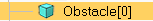
\includegraphics[scale=1.0, angle=0]{Images/tarea2/detectable_1.png} \\
    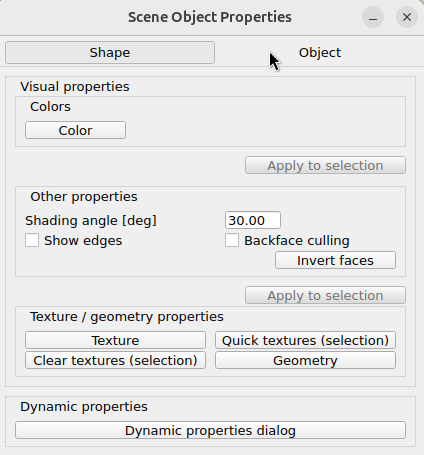
\includegraphics[scale=0.48, angle=0]{Images/tarea2/detectable_2.png}
    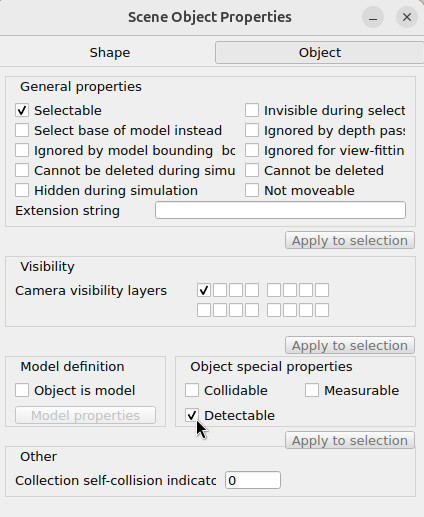
\includegraphics[scale=0.42, angle=0]{Images/tarea2/detectable_3.png}
    \caption{\label{fig:t2.detectable} Cómo marcar un objeto como detectable.}
    \end{center}
\end{figure}

\begin{figure}[H]
    \begin{center}
    %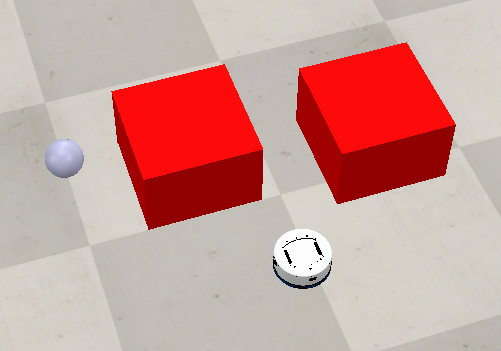
\includegraphics[scale=0.346, angle=0]{Images/tarea2/escenario1.png}
    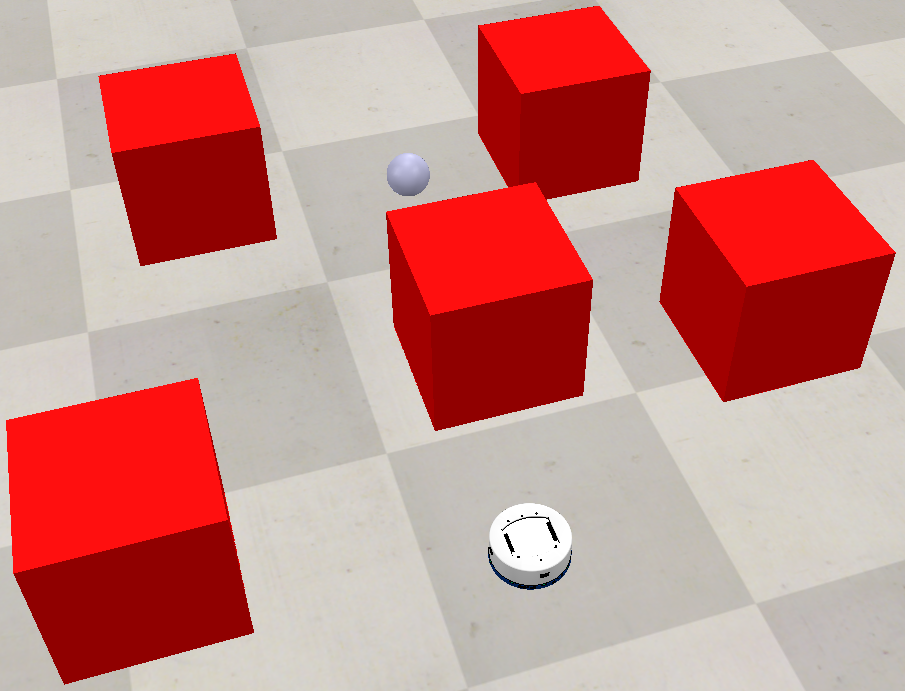
\includegraphics[scale=0.175, angle=0]{Images/tarea2/escenario2.png}
    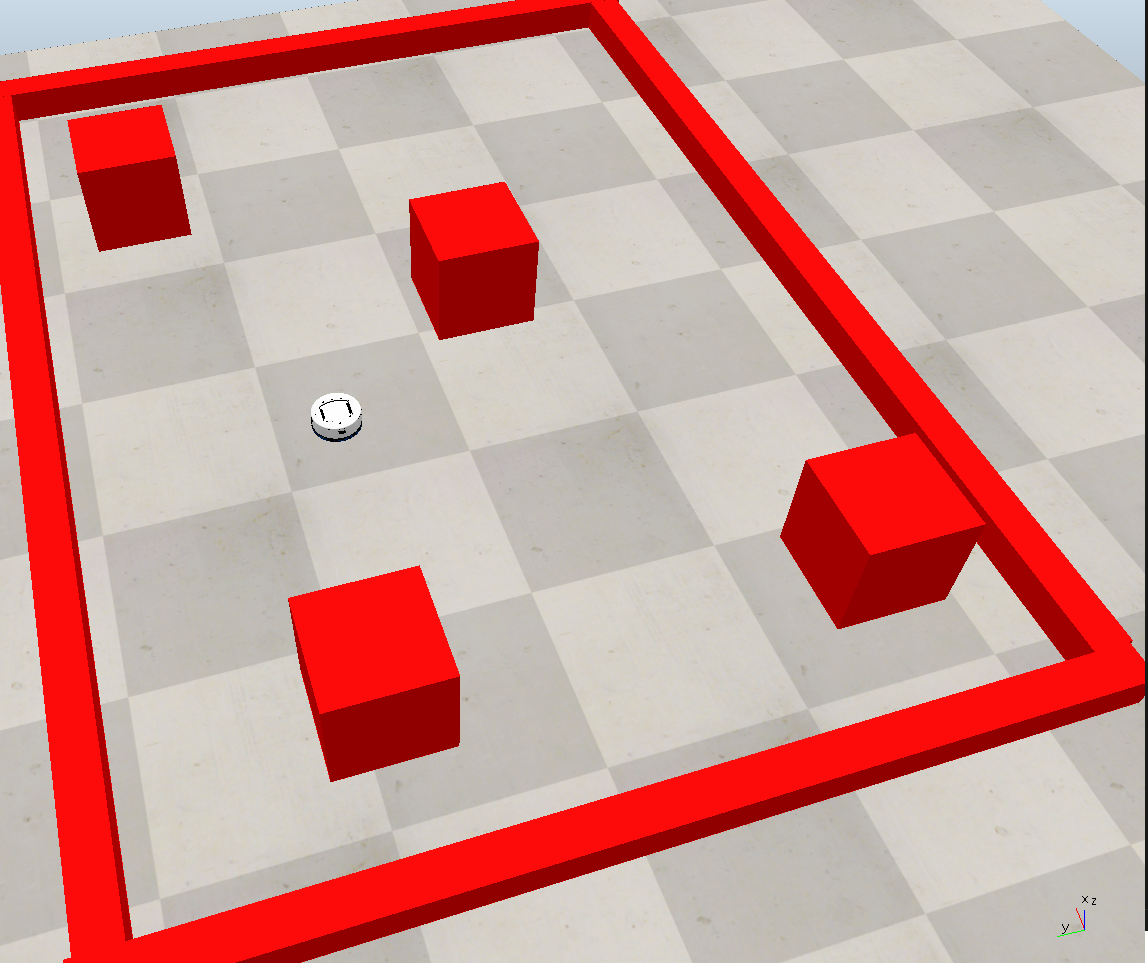
\includegraphics[scale=0.125, angle=0]{Images/tarea2/escenario3.png}
    \caption{\label{fig:t2.escenario} Escenarios propuestos para la segunda tarea.}
    \end{center}
\end{figure}

\subsection*{2. Implementar el algoritmo de \textit{Braitenberg} por medio de la manipulación de
las velocidades del robot.}
\addcontentsline{toc}{subsection}{2. Implementar el algoritmo de \textit{Braitenberg} por medio de la manipulación de
las velocidades del robot.}

El algoritmo de \textit{Braitenberg} se refiere a aquellos procesos
de control de vehículos reactivos (o de \textit{Braitenberg}) que relacionan directamente señales
sensoriales a actuadores mediante ganancias simples, generando
comportamientos complejos a partir de reglas locales \cite{braitenberg1984vehicles}.
En otras palabras,
el concepto de vehículos de \textit{Braitenberg} corresponde a aquellos 
cuyos actuadores están directamente gobernados por los sensores, esto es,
los sensores están conectados a los actuadores. \\

Este esquema describe comportamientos reactivos y en la práctica, 
esto se implementa mapeando lecturas de sensores \(s_i\) 
a comandos de ruedas mediante matrices de ganancia, sin 
planificación ni memoria interna.\\

En la Figura \ref{fig:t2.braitenberg}
se ilustran estos vehículos, 
donde las flechas de color negro representan la conexión directa \texttt{sensor} 
$\rightarrow$ \texttt{actuador}, mientras que la de color azul el movimiento
reactivo del robot según la lectura de los sensores. El círculo de color 
rojo representa un obstáculo a esquivar.\\

\begin{figure}[H]
    \begin{center}
    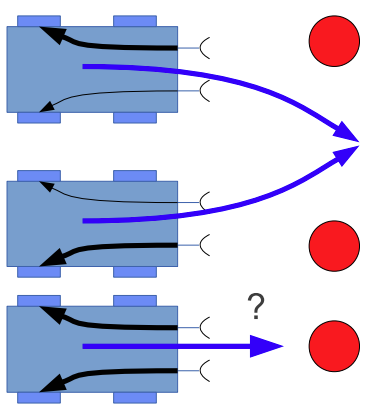
\includegraphics[scale=0.5, angle=0]{Images/tarea2/braitenberg.png}
    \caption{\label{fig:t2.braitenberg} Vehículos de \textit{Braitenberg}
    \cite{dicaro2017behaviors}.}
    \end{center}
\end{figure}

Un esquema \textit{Braitenberg} clásico para un robot diferencial se expresa como
\begin{equation}
  v_L \;=\; \sum_{i} G_{L,i}\,f(s_i), \qquad
  v_R \;=\; \sum_{i} G_{R,i}\,f(s_i),
  \label{eq:braitenberg}
\end{equation}
donde \(G_{L,i},G_{R,i}\) son las ganancias que conectan el 
sensor \(i\) con las ruedas, \(f(\cdot)\) es el preprocesado
(inversión, saturación, normalización, filtrado, etc.) y \(v_L,v_R\) 
son las velocidades lineales de las ruedas (m/s). \\

La velocidad lineal del chasis \(v\) y su velocidad angular
\(\omega\) se obtienen de las Ecuaciones \ref{eq:2} o \ref{eq:3}. 
Como el robot controla los motores mediante velocidades angulares 
de rueda, las velocidades lineales de rueda se convierten a 
velocidades angulares mediante el radio de rueda \(r\), Ecuaciones \ref{eq:22},
obteniendo así las Ecuaciones \ref{eq:2}.

\begin{equation}
  \omega_L \;=\; \frac{v_L}{r}, \qquad
  \omega_R \;=\; \frac{v_R}{r}.
  \label{eq:22}
\end{equation}

Existen dos estrategias principales para la implementación de este enfoque:
\begin{itemize}
  \item \textbf{Conexión directa (clásica)}: cada sensor contribuye linealmente a las ruedas.
  \item \textbf{Contralateral}: sensores frontales izquierdos conectan a la rueda derecha y viceversa.
\end{itemize}

Asimismo, en función del caso de uso se pueden sugerir variantes, como la conexión de un sensor 
a su correspondiente rueda lateral con signo invertido para comportamientos de atracción, 
ponderación de cada sensor para evitar que una lectura domine o la combinación con controladores de
objetivo con sintonización de las ganancias. \\

De esta manera, en esta tarea se implementan dos controladores con esquivación del obstáculos. 
El primero es una esquivación de obstáculos sin un objetivo de posición a alcanzar. El 
segundo combina el control de posición de la primera tarea con la esquivación de obstáculos 
\textit{Braitenberg}, para el que se ha tenido que modificar el esquema clásico de \textit{Braitenberg}.

La información de posición de los obstáculos respecto del robot viene dada por los 
ocho sensores infrarrojos que incorpora el robot en uso. Estos sensores generan 
un valor de distancia comprendido en el rango $[0.002, 0.25]$ metros \cite{kheperaiv_manual_rev3}.
Los sensores están distribuidos alrededor del chasis separados angularmente por 45$^\circ$, 
de forma que es capaz de obtener información en 360$^\circ$. \\

En \textit{CoppeliaSim}, cuando se solicita a uno de los sensores su lectura,
devuelve dos valores: \textit{detected}, \textit{distance}. El primero de ellos
puede tomar los valores $0$ o $1$, e indica si se ha producido una detección o no, es 
decir, si no hay ningún objeto dentro del rango de operación del sensor, este valor 
será $0$. También podría ocurrir que el objeto esté dentro de dicho rango, 
pero que por luminosidad o reflectancia, por ejemplo, no sea capaz de detectarlo,
aunque esta situación queda fuera del alcance de este trabajo. En cuanto al segundo,
contiene la distancia detectada al obstáculo. \\

Continuando con la arquitectura presentada en la primera tarea, se ha definido en el 
robot del simulador el script \textit{Lua} \texttt{publisher\_infrared},
Código \ref{cod:t2_pubInfrared}, que genera un tópico
\textit{ROS2} por cada sensor infrarrojo. Estos tópicos, \texttt{/khepera/ir1},
\texttt{/khepera/ir2}, \texttt{/khepera/ir3}, \texttt{/khepera/ir4}, 
\texttt{/khepera/ir5}, \texttt{/khepera/ir6}, \texttt{/khepera/ir7} y 
\texttt{/khepera/ir8}, transportan el mensaje de tipo \texttt{sensor\_msgs/msg/Range}.
Su documentación está en el enlace \url{https://docs.ros.org/en/jazzy/p/sensor_msgs/msg/Range.html}. \\

Los campos de dicho mensaje más relevantes para este trabajo son los siguientes:
\textit{radiation\_type}, $0$ si se usan sensores ultrasónicos y $1$ si se usan infrarrojos;
\textit{min\_range} y \textit{max\_range}, límites del rango de operación de los sensores 
en uso; y \textit{range}, distancia obtenida por el sensor. \\

Además, es fundamental procesar los valores de aquellos sensores que no detecten 
obstáculos, puesto que el simulador los establece a cero. Este comportamiento 
supone un problema a la hora de esquivar obstáculos, por lo que se debe establecer 
el campo \textit{range} de estos sensores al límite superior de detección, en este caso,
$0.25$ metros.


\subsubsection*{2.1 Controlador \textit{Braitenberg} sin posición objetivo.}
Este controlador sigue el esquema reactivo clásico de las Ecuaciones \ref{eq:braitenberg}. 
Está diseñado para evitar obstáculos sin perseguir una meta explícita, esto es,
que el robot esté en movimiento continuo sin colisionarse mediante la 
esquivación eficaz de los objetos y las paredes. Por ello, 
este sistema opera sobre el escenario de la Figura \ref{fig:t2.escenario1}, 
que consta de un entorno cerrado por paredes y cuatro obstáculos repartidos 
por el terreno.

\begin{figure}[H]
    \begin{center}
    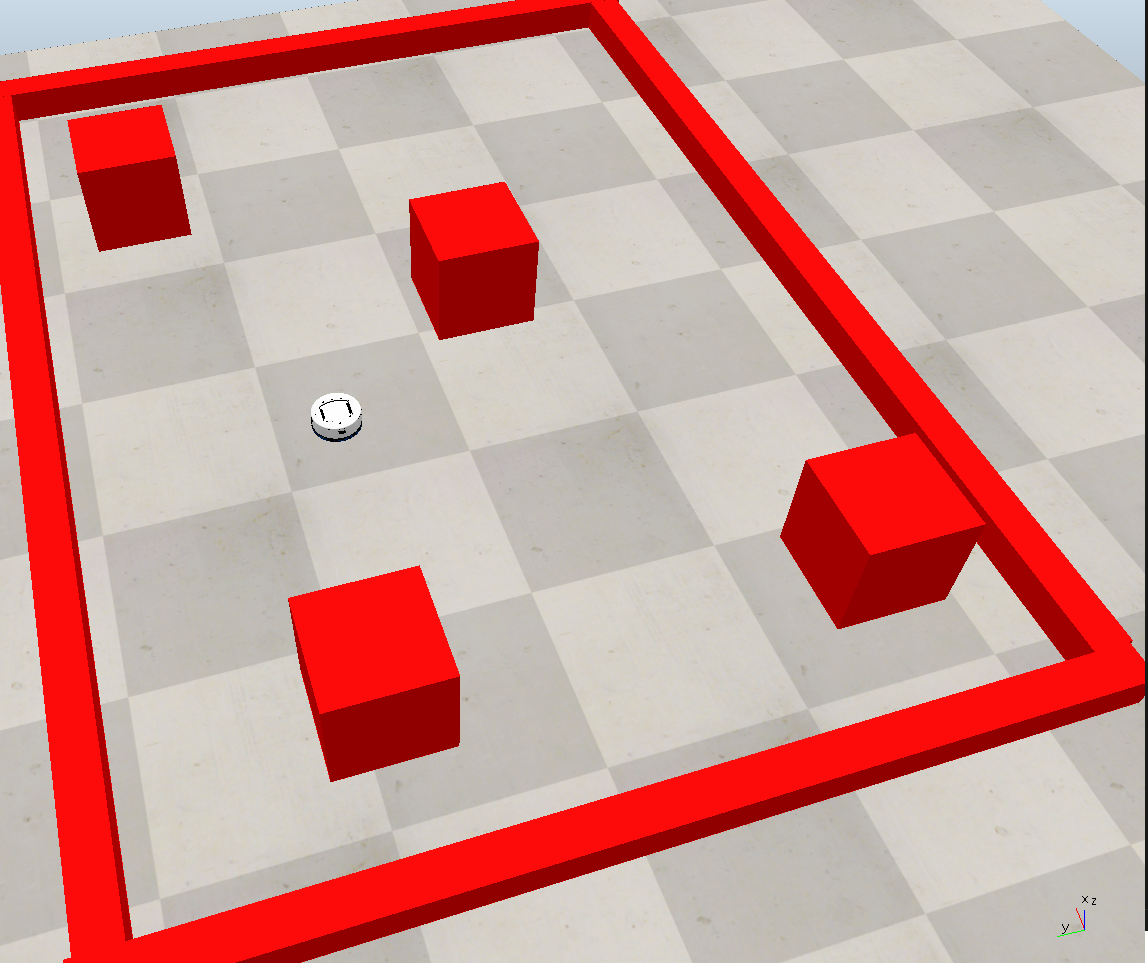
\includegraphics[scale=0.3, angle=0]{Images/tarea2/escenario3.png}
    \caption{\label{fig:t2.escenario1} Escenario para el primer controlador
    \textit{Braitenberg}.}
    \end{center}
\end{figure}

La entrada sensorial proviene de los ocho sensores mencionados.
Cada lectura se preprocesa y normaliza a una señal de detección
 \(\mathrm{detect}_i\in[0,1]\) mediante una inversión lineal entre el umbral mínimo
 y máximo de detección:
\begin{equation}
\mathrm{detect}_i \;=\; \operatorname{clamp}\!\left(1 - \frac{d_i - d_{\min}}{d_{\max}-d_{\min}},\,0,1\right),
\label{eq:detect}
\end{equation}

donde \(d_{\min}=\) \texttt{max\_detection\_dist}, es decir,
la distancia a partir de la que el sensor produce la máxima activación (repulsión = 1.0)
y \(d_{\max}=\) \texttt{max\_range\_default}, esto es, el límite superior de operación
del sensor: $0.25$ metros. 
Las lecturas inválidas o fuera de rango se sustituyen por \(d_{\max}\). \\


Las velocidades lineales de rueda se calculan ampliando el esquema de las 
Ecuaciones \ref{eq:braitenberg} al añadir una velocidad base \(v_0\), Ecuaciones
\ref{eq:braitenberg2}. Esta velocidad base permite que al robot avanzar en línea 
recta cuando no se encuentra rodeado de obstáculos. Además, para garantizar la 
seguridad operativa estas velocidades calculadas
se saturan con los límites configurados, Ecuaciones \ref{eq:braitenberg_sat}.

\begin{equation}
v_{L,\text{lin}} \;=\; v_0 \;+\; \sum_{i=1}^{8} G_{L,i}\,\mathrm{detect}_i,\qquad
v_{R,\text{lin}} \;=\; v_0 \;+\; \sum_{i=1}^{8} G_{R,i}\,\mathrm{detect}_i.
\label{eq:braitenberg2}
\end{equation}

\begin{equation}
v_{L,\text{lin}} \leftarrow \operatorname{clamp}(v_{L,\text{lin}},\, v_{\min},\, v_{\max}),\qquad
v_{R,\text{lin}} \leftarrow \operatorname{clamp}(v_{R,\text{lin}},\, v_{\min},\, v_{\max}).
\label{eq:braitenberg_sat}
\end{equation} 

Se han utilizado los vectores de ganancias expuestos en las Ecuaciones \ref{eq:ganancias},
que implementan un control contralateral. El orden de los sensores es el siguiente:
trasero izquierdo, izquierdo, frontal izquierdo, frontal, frontal derecho,
derecho, trasero derecho, trasero. Presentan una estructura simétrica donde 
los sensores frontales y laterales ejercen mayor influencia, 
mientras que los sensores traseros tienen pesos muy reducidos. \\

En el caso de la rueda izquierda (vector $GL$), los sensores situados en el
semiplano derecho del robot —frontal derecho, derecho y trasero derecho— poseen
ganancias negativas. Esto provoca que, ante la detección de un obstáculo en la 
derecho, la rueda izquierda reduzca su velocidad, generando un giro hacia la izquierda 
que aleja al robot del obstáculo. De forma análoga, en el vector $GR$ los sensores del
semiplano izquierdo —frontal izquierda, izquierdo y trasero izquierdo— presentan
ganancias negativas, induciendo un giro hacia la derecha cuando se detectan obstáculos
en la izquierda. \\

Los sensores frontales (índices 2, 3 y 4) tienen las ganancias de mayor magnitud,
lo que refuerza la reacción ante obstáculos frontales en la trayectoria del robot. 
En ambos casos se ha decidido anular la acción de los sensores traseros, puesto que 
el robot se desplaza hacia adelante y así se evitan sobreimpulsos repulsivos.

\begin{equation}
\begin{aligned}
GL: &[0.0,0.0,0.0,0.0,-0.05,-0.075,-0.1,-0.00125] \\
GR: &[-0.00125,-0.1,-0.075,-0.05,0.0,0.0,0.0,0.0]
\end{aligned}
\label{eq:ganancias}
\end{equation} 
Las ganancias se han ajustado mediante ensayo y error \cite{braitenberg_video}. \\

Finalmente, la cinemática diferencial del chasis convierte las velocidades
de rueda en velocidad lineal \(V\) y velocidad angular \(\omega\) del robot mediante
las Ecuaciones \ref{eq:3} y \ref{eq:22}. \\

Las velocidades de chasis se publican como un mensaje \texttt{geometry\_msgs::msg::Twist} 
con \(\text{linear.x}=V\) y \(\text{angular.z}=\omega\) a través del tópico \texttt{/cmd\_vel}. \\

En la Figura \ref{fig:t2_rdo_traj} se presenta la trayectoria resultante sobre el escenario 
propuesto durante el primer minuto de ejecución, donde se aprecia claramente que el 
algoritmo implementado dota al robot de la capacidad de esquivar los obstáculos.
En la Figura \ref{fig:t2_rdo_vels} se muestran las velocidades lineal y angular del robot
durante la trayectoria anterior, donde se observa que cuando no hay obstáculos detectados
el robot se desplaza a $0.1 m/s$ y sin velocidad angular. Estos resultados se han 
obtenido con los parámetros del Código \ref{cod:t2.params_1}. \\

Para ejecutar el controlador, una vez esté cargado el escenario en \textit{CoppeliaSim}
y la simulación en ejecución, ejecutar el siguiente comando:
\texttt{ros2 run tarea2 braitenberg\_puro --ros-args --params-file src/tarea2/config/params.yaml}. 

\begin{figure}[H]
    \begin{center}
    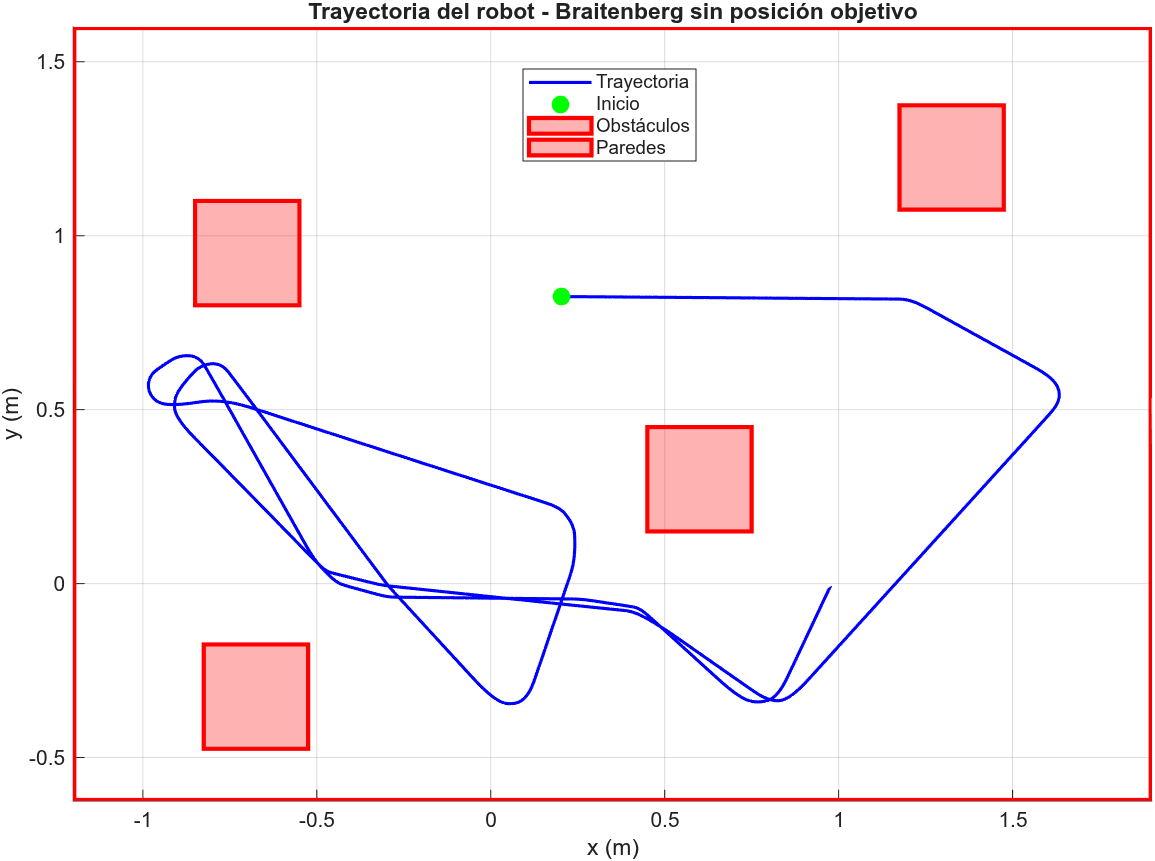
\includegraphics[scale=0.7, angle=0]{Images/tarea2/braitenberg1/traj.png}
    \caption{\label{fig:t2_rdo_traj} Trayectoria realizada por el robot con el primer controlador
    \textit{Braitenberg}.}
    \end{center}
\end{figure}

\begin{figure}[H]
    \begin{center}
    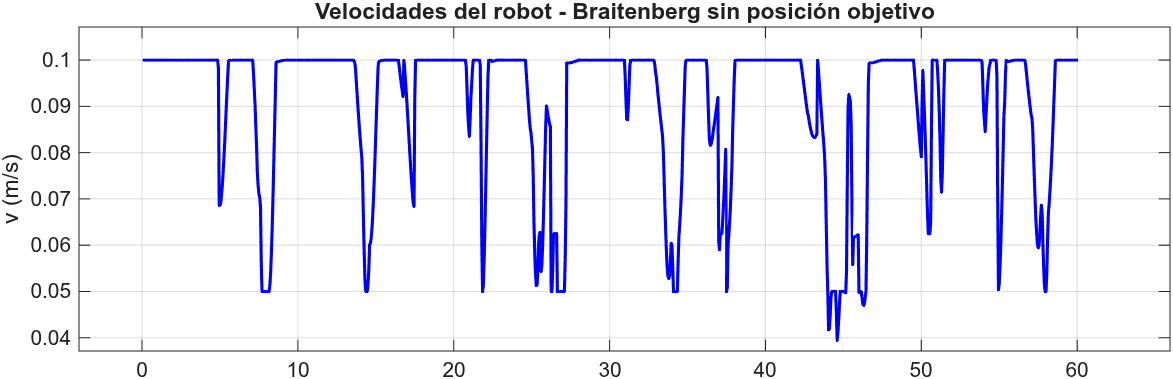
\includegraphics[scale=0.8, angle=0]{Images/tarea2/braitenberg1/v.png} \\
    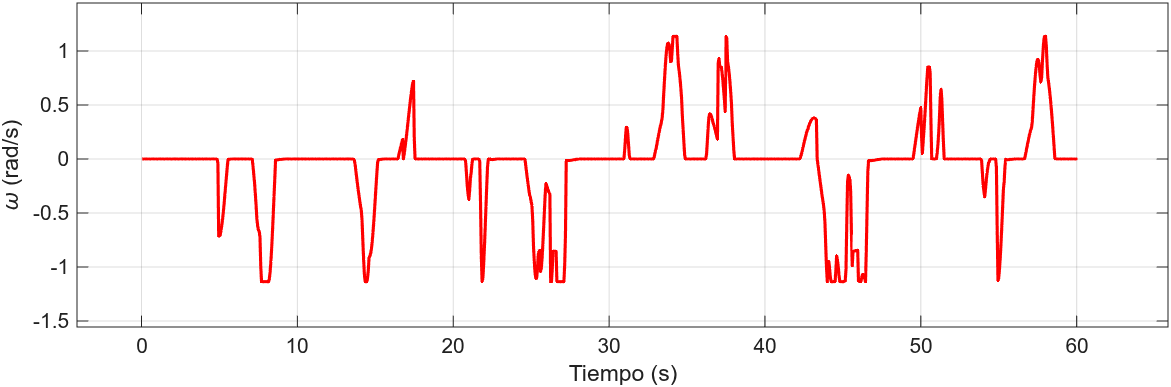
\includegraphics[scale=0.8, angle=0]{Images/tarea2/braitenberg1/w.png}
    \caption{\label{fig:t2_rdo_vels} Velocidades lineal y angular del robot
    durante la trayectoria del primer controlador \textit{Braitenberg}.}
    \end{center}
\end{figure}

\clearpage

%%%%%
%%%%%
%%%%%

\subsubsection*{2.2 Controlador \textit{Braitenberg} con posición objetivo.}
Este controlador buscar combinar el control de posición de la primera tarea 
con la esquivación de obstáculos mediante el algoritmo de \textit{Braitenberg}.
Por tanto, su objetivo es desplazarse hasta una posición objetivo esquivando
obstáculos. Este sistema opera sobre los escenarios de la Figura \ref{fig:t2.escenario2}, 
que consta de un entorno cerrado por paredes y cuatro obstáculos repartidos 
por el terreno.

\begin{figure}[H]
    \begin{center}
    %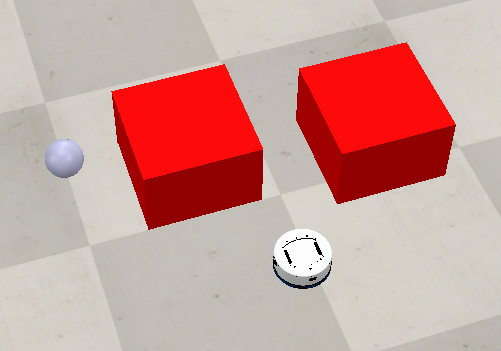
\includegraphics[scale=0.4, angle=0]{Images/tarea2/escenario1.png}
    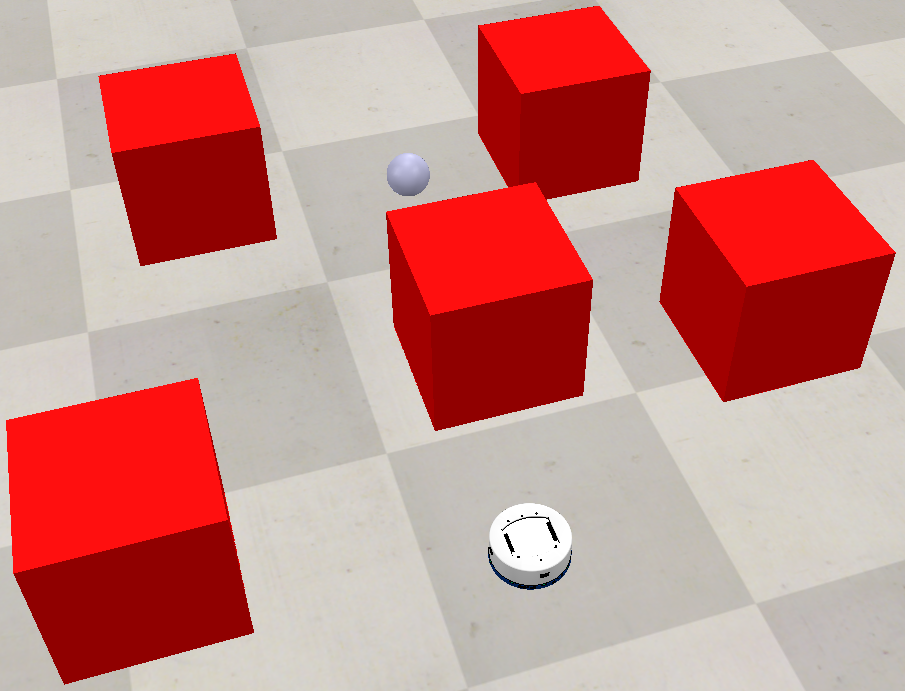
\includegraphics[scale=0.203, angle=0]{Images/tarea2/escenario2.png}
    \caption{\label{fig:t2.escenario2} Escenario para el segundo controlador
    \textit{Braitenberg}.}
    \end{center}
\end{figure}

Un aspecto fundamental de este controlador respecto del anterior es la modificación
en el esquema de \textit{Braitenberg}. El controlador de posición genera una
intención de movimiento \((V_{\text{goal}},\omega_{\text{goal}})\) que busca reducir
el error de posición y orientación. El esquema clásico de \textit{Braitenberg} que 
actúa directamente sobre las velocidades de rueda introduce una corrección de alta
frecuencia y granular que puede contradecir instantáneamente la intención del
controlador de posición. Esa contradicción se manifiesta como un lazo de 
realimentación no deseado donde la corrección reactiva cambia la orientación y posición, 
el controlador de posición responde cambiando la intención, y la repulsión vuelve
a reaccionar, produciendo oscilaciones alrededor de la trayectoria prevista e incluso 
estancamientos. \\

Asimismo, la conexión directa clásica de los sensores con los actuadores lo hace 
especialmente sensible al ruido pudiendo generar picos aislados, lo que se traduce 
en giros bruscos y rápidos cambios de signo en la velocidad angular. \\

También existen incompatibilidades entre magnitudes. El enfoque clásico 
actúa sobre las velocidades lineales de los actuadores, mientras que el 
controlador de posición implementado en la primera tarea actúa sobre la 
velocidad lineal y angular del chasis del robot. Por tanto, es altamente 
recomendable diseñar un esquema de \textit{Braitenberg} que funcione 
sobre las velocidades del chasis del robot. \\

Consecuentemente, se propone el siguiente esquema.

\paragraph{Funciones de activación}
Sea \(r_i\) la lectura del sensor \(i\) ($a_0$: trasero izquierdo, $a_1$: izquierdo,
$a_2$: frontal izquierdo, $a_3$: frontal, $a_4$: frontal derecho,
$a_5$: derecho, $a_6$: trasero derecho, $a_7$: trasero), se define la activación
normalizada por sensor como
\begin{equation}
a_i \;=\; \operatorname{clamp}\!\left(1 - \frac{r_i}{r_{\max}},\,0,1\right),
\label{eq:act}
\end{equation}
donde \(r_{\max}=0.25\ \mathrm{m}\). Aquellos sensores que no detecten objeto, 
marcarán $r_i$ como $0.25$, y por tanto, su activación será $0$, puesto que no 
tienen que generar ninguna repulsión. De forma análoga, si detectan un obstáculo 
se genera una activación lineal a la distancia hasta el objeto.

\paragraph{Agregación zonal}
Se agrupan las activaciones en tres zonas (frontal, izquierda y derecha):
\begin{equation}
A_{\text{front}}=\frac{a_{2}+a_3+a_{4}}{3},\qquad
A_{\text{left}}=\frac{a_{2}+a_1}{2},\qquad
A_{\text{right}}=\frac{a_{4}+a_5}{2}.
\label{eq:agreg}
\end{equation}

Se descarta el uso de los sensores traseros porque el robot se mueve hacia adelante,
por lo que nunca se encontrará con obstáculos por detrás. Podría darse 
el caso de que los obstáculos fuesen móviles y dinámicos y se acercasen por detrás 
al robot. No obstante, el planteamiento de este controlador es que esos obstáculos
implementasen también la esquivación de obstáculos, ya que esquivar objetos que 
se encuentran en dirección opuesto al objetivo de posición sería contraproducente.

\paragraph{Componentes reactivas no lineales}
Las salidas reactivas en el espacio del chasis se definen como
\begin{equation}
v_{\text{react}} \;=\; -\,k_{\text{front}}\;A_{\text{front}}^{p},
\qquad
\omega_{\text{react}} \;=\; k_{\text{turn}}\;\tanh\!\big(A_{\text{right}}-A_{\text{left}}\big),
\label{eq:react}
\end{equation}
con \(k_{\text{front}}>0,\;k_{\text{turn}}>0\) y exponente \(p\geq 1\) 
(en la implementación \(k_{\text{front}} = 1.6,\; k_{\text{turn}} = 4.0,\; p=1.5\)). La potencia en \(A_{\text{front}}\) prioriza 
reacciones fuertes sólo en proximidades críticas y la función \(\tanh\), 
Figura \ref{fig:t2.tanh}, introduce una no linealidad suave y limitada y permite 
convertir la diferencia de activaciones laterales en una antivación angular 
acotada y continua en el rango $[-1, 1]$, evitando saturaciones abruptas y centrando
la salida en cero.

\begin{figure}[H]
    \begin{center}
    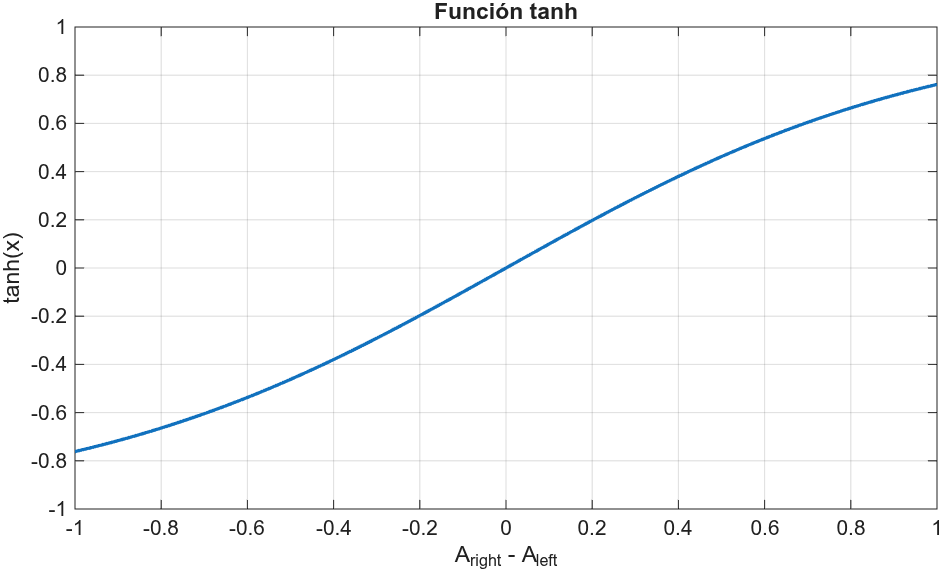
\includegraphics[scale=0.85, angle=0]{Images/tarea2/tanh.png}
    \caption{\label{fig:t2.tanh} Función \(tanh(x)\).}
    \end{center}
\end{figure}


\paragraph{Escalado proporcional a la distancia al objetivo}
Para mantener coherencia de magnitudes con el controlador de posición se aplica
un factor de escala dependiente de la distancia al objetivo ($d$):
\begin{equation}
\mathrm{factor} \;=\; \operatorname{clamp}\!\left(\frac{d}{k_s},\,0,1\right),
\label{eq:scale}
\end{equation}
donde $d$ es la distancia instantánea al objtivo de posición y $k_s$
el parámetro de escala que representa la distancia de referencia
(en la implementación $k_s = 1.0$). \\

Si $k_s > 1$ entonces la escala crece más despacio con la distancia. Para 
$d < k_s$ la parte reactiva está atenuada y solo cuando $d < k_s$
la reacción se aplica al 100\%. El efecto que se obtiene es otorgar mayor
prioridad al control hacia el objetivo en distancias intermedias y
reacciones fuertes solo cuando el robot está lejos del objetivo. \\

Si $k_s = 1$ entonces la escala es proporcional a $d$ hasta un máximo de $1$ 
proporcionando equilibrio directo entre distancia en metros y respuesta reactiva. \\

Si $k_s < 1$ entonces la escala alcanza 1 con distancias pequeñas. Para 
$d ≥ k_s$ la repulsión se aplica por completo incluso relativamente cerca del objetivo. 
Por tanto, la parte reactiva tiene mayor influencia incluso a distancias cortas. \\

Después, se combinan las salidas del controlador de posición, $v_{\text{goal}}$
y $\omega_{\text{goal}}$, con las salidas de la repulsión de \textit{Braitenberg},
$v_{\text{react}}$ y $\omega_{\text{react}}$, mediante las Ecuaciones \ref{eq:t2_v_final}.

\begin{equation}
v \;=\; v_{\text{goal}}\, + \mathrm{factor}\cdot v_{\text{react}},\qquad
\omega \;=\; \omega_{\text{goal}}\, + \mathrm{factor}\cdot \omega_{\text{react}}
\label{eq:t2_v_final}
\end{equation}

Por último, se saturan ambas velocidades. La lineal, al rango $[0, v_{\text{max}}]$ y 
la angular, al rango $[\omega_{\text{max}}, \omega_{\text{max}}]$. Si se desea 
que el robot no se detenga en ninguna situación, el límite inferior de la saturación
de la velocidad lineal tendrá que establecerse a $v_{\text{min}}$. Sin embargo,
esta situación dificultaría la repulsión. \\

En las Figuras \ref{fig:t2_rdo_target1} y \ref{fig:t2_rdo_target2} se presenta 
la trayectoria resultante sobre el escenario propuesto
con los controladores de posición reactivo y geométrico.
Se observa que el algoritmo implementado es capaz de guiar al robot hasta 
la posición objetivo esquivando los obstáculos, obteniendo mejores resultados 
con el controlador de posición reactivo. Este resultado es coherente con la 
naturaleza de cada sistema, ya que el controlador basado en curvatura 
intenta moverse dibujando un arco de circunferencia, generando una restricción adicional
y por tanto, dificultando la gobernanza del robot entre obstáculos. En la Tabla
\ref{tab:controladores_brai_desempeno} se presentan estos resultados de manera 
analítica mediante las cuatro métricas de evaluación empleadas en la primera tarea, 
donde se ha coloreado en amarillo los valores más bajos obtenidos para cada métrica.

\begin{table}[H]
  \centering
\begin{tabular}{|c|c|c|}
\hline
\multicolumn{1}{|l|}{\textbf{}} & \textbf{Reactivo}            & \textbf{Geométrico} \\ \hline
\textbf{IAE}                    & \cellcolor[HTML]{FFFE65}6.14 & 7.34               \\ \hline
\textbf{ISE}                    & \cellcolor[HTML]{FFFE65}4.30 & 5.03                \\ \hline
\textbf{ITAE}                   & \cellcolor[HTML]{FFFE65}24.46 & 35.34                \\ \hline
\textbf{ITSE}                   & \cellcolor[HTML]{FFFE65}12.15 & 17.28                \\ \hline
\end{tabular}
\caption{Evaluación de los controladores \textit{Braitenberg} con control de posición.}
\label{tab:controladores_brai_desempeno}
\end{table}

En las Figuras \ref{fig:t2_rdo_targetVel1} y \ref{fig:t2_rdo_targetVel2} se muestran 
las velocidades lineal y angular del robot
durante las trayectorias anteriores, donde también se observa que para este caso de uso 
el controlador de posición basado en curvatura es más inestable. Estos resultados se han 
obtenido con los parámetros del Código \ref{cod:t2.params_2}. \\

Para ejecutar el controlador, una vez esté cargado el escenario en \textit{CoppeliaSim}
y la simulación en ejecución, ejecutar el siguiente comando:
\texttt{ros2 run tarea2 braitenberg\_target\_controller --ros-args --params-file src/tarea2/config/params.yaml}. 
Y al igual que con la primera tarea, es necesario solicitar la ejecución de la acción
mediante el comando del Código \ref{cod:actionClient}, a través del que se indica 
la posición objetivo.

\begin{figure}[htb]
    \begin{center}
    
\includegraphics[scale=0.95, angle=0]{Images/tarea2/braitenberg2/traj1.png}
    \caption{\label{fig:t2_rdo_target1} Trayectoria realizada por el robot con el segundo controlador
    \textit{Braitenberg} con control de posición reactivo.}
    \end{center}
\end{figure}

\begin{figure}[htb]
    \begin{center}
    
\includegraphics[scale=0.95, angle=0]{Images/tarea2/braitenberg2/traj2.png}
    \caption{\label{fig:t2_rdo_target2} Trayectoria realizada por el robot con el segundo controlador
    \textit{Braitenberg} con control de posición geométrico.}
    \end{center}
\end{figure}

\begin{figure}[htb]
    \begin{center}
    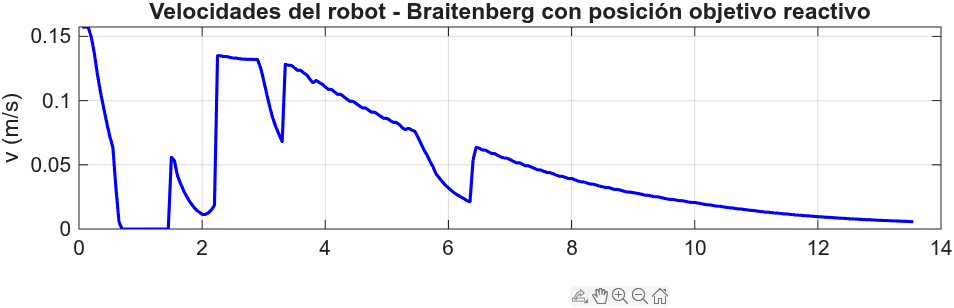
\includegraphics[scale=0.8, angle=0]{Images/tarea2/braitenberg2/v_1.png} \\
    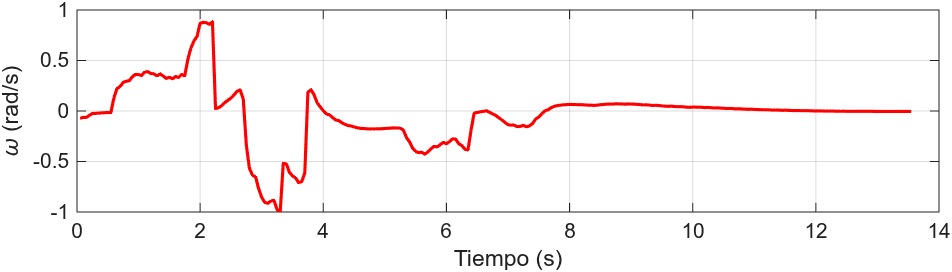
\includegraphics[scale=0.8, angle=0]{Images/tarea2/braitenberg2/w_1.png}
    \caption{\label{fig:t2_rdo_targetVel1} Velocidades lineal y angular del robot
    durante la trayectoria del segundo controlador \textit{Braitenberg} con 
    control de posición reactivo.}
    \end{center}
\end{figure}

\begin{figure}[htb]
    \begin{center}
    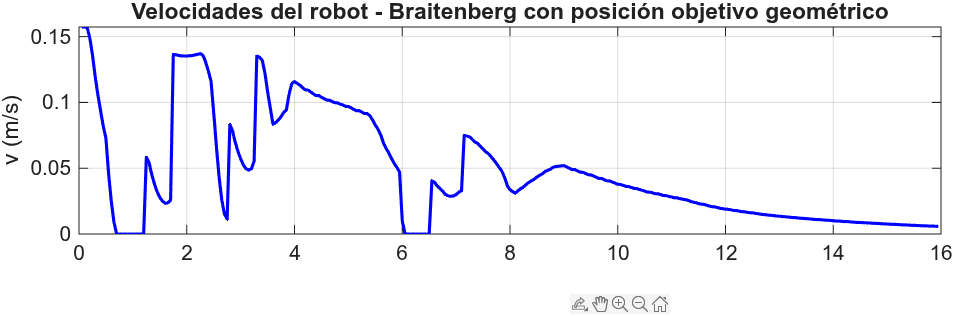
\includegraphics[scale=0.8, angle=0]{Images/tarea2/braitenberg2/v_2.png} \\
    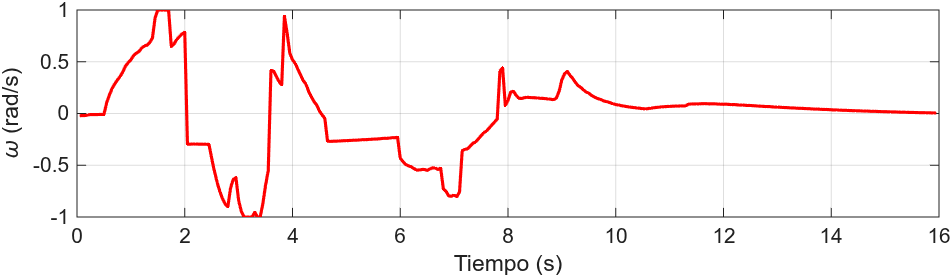
\includegraphics[scale=0.8, angle=0]{Images/tarea2/braitenberg2/w_2.png}
    \caption{\label{fig:t2_rdo_targetVel2} Velocidades lineal y angular del robot
    durante la trayectoria del segundo controlador \textit{Braitenberg} con 
    control de posición reactivo.}
    \end{center}
\end{figure}